\begin{enumerate}[(a)]
	\item 

        \begin{figure}[H]
        \centering
        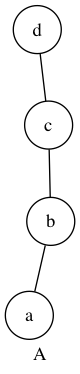
\includegraphics[scale=0.5]{118/1.png}
        \end{figure}

        \begin{figure}[H]
        \centering
        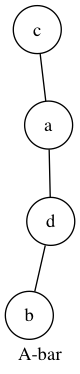
\includegraphics[scale=0.5]{118/1i.png}
        \end{figure}

        \begin{figure}[H]
        \centering
        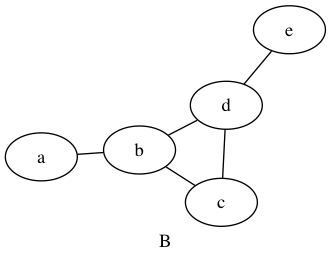
\includegraphics[scale=0.5]{118/2.png}
        \end{figure}

        \begin{figure}[H]
        \centering
        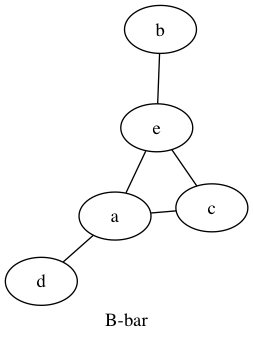
\includegraphics[scale=0.5]{118/2i.png}
        \end{figure}

        \begin{figure}[H]
        \centering
        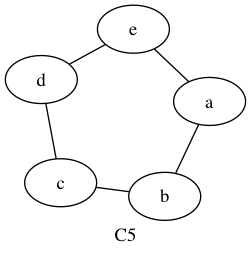
\includegraphics[scale=0.5]{118/3.png}
        \end{figure}

        \begin{figure}[H]
        \centering
        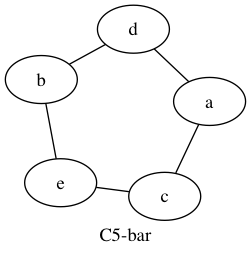
\includegraphics[scale=0.5]{118/3i.png}
        \end{figure}

	\item Consider the number of two element subsets of $V(G)$. Clearly this
		is $n(n-1)/2$. Now each of these two element subsets is an edge in precisely
		one of $G$ and $\overline{G}$. So $n(n-1)/2=|E(G)|+|E(\overline{G})|$.
	But if $G \cong \overline{G}$, then $m=|E(G)|=|E(\overline{G})|$, so
	$n(n-1)/2=2m$, or $n(n-1)=4m$, and $4|n(n-1)$. But $gcd(n,n-1)=1$, so $4|n$ or
	$4|n-1$, so $n$ is $0$ or $1$ modulo $4$.
\end{enumerate}
